\subsection{Painting rectification of the 3D model}

For the painting rectification of the 3D model, we manage to replace the low quality painting images with a rectified version of the same paintings in higher quality, retrieved from the database. Given a screenshot from the 3D model, it goes through the first part of our pipeline until the correspondent painting is found. The retrieved painting is subject to a projective transformation, with an inverse process w.r.t our main pipeline, in order for it to have the same projection as the painting in the screenshot. It is, then, replaced in the screenshot with the use of a mask. If the painting is not found, the warping is not performed. An example can be seen in fig.~\ref{fig:3d-warping}.

\begin{figure}[h!]
  \centering
  \resizebox{0.45\textwidth}{!}{
  \resizebox{0.809\textwidth}{!}{\minipage{0.3\textwidth}
      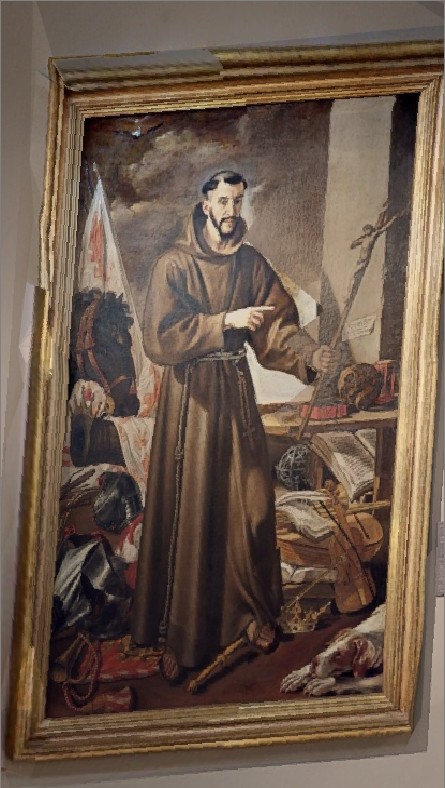
\includegraphics[width=\linewidth]{pictures/painting_detection/3d_rectification_original.PNG}
      \caption*{Original 3D model painting}\label{fig:rectification_original}
    \endminipage\hfill}
    \resizebox{0.8\textwidth}{!}{\minipage{0.3\textwidth}
      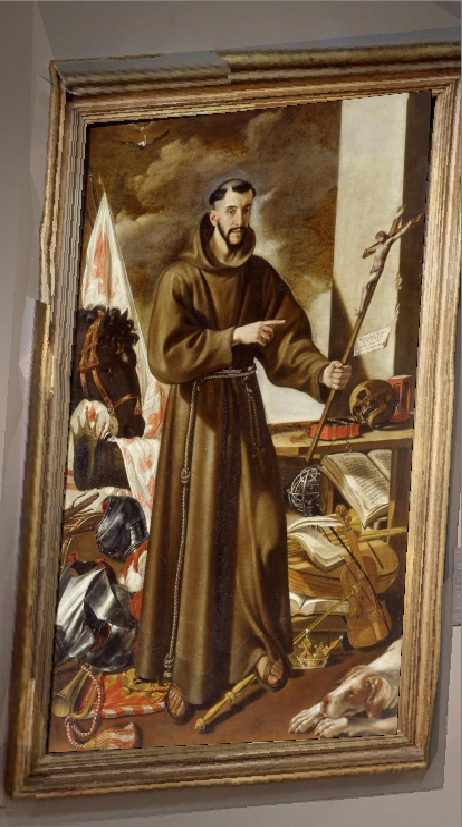
\includegraphics[width=\linewidth]{pictures/painting_detection/3d_rectification_warped.PNG}
      \caption*{Replaced painting}\label{fig:rectification_warped}
    \endminipage\hfill}}
    \caption{Painting rectification from the 3D view.}\label{fig:3d-warping}
\end{figure}




